\section{Правильные многоугольники}

\paragraph{}\label{1938/212}
\so{Определения}.
Ломаная линия называется правильной, если она удовлетворяет следующим трём условиям:
1) отрезки прямых, составляющие её, равны;
2) углы, составленные каждыми двумя соседними отрезками, равны;
3) из каждых трёх последовательных отрезков первый и третий расположены по одну сторону от прямой, на которой лежит второй.

\begin{figure}[h]
\centering
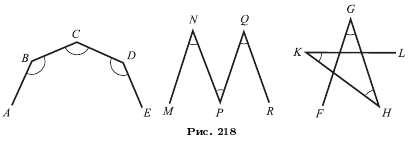
\includegraphics{mppics/ris-218}
\caption{}\label{1938/ris-218}
\end{figure}

Таковы, например, линии $ABCDE$ и $FGHKL$ (рис.~\ref{1938/ris-218});
но ломаную $MNPQR$ нельзя назвать правильной, потому что она не удовлетворяет третьему условию.

Правильная ломаная может быть \rindex{выпуклая ломаная}\textbf{выпуклой}, как например линия $ABCDE$.

Многоугольник называется \rindex{правильный многоугольник}\textbf{правильным}, если он ограничен правильной ломаной линией, то есть если он имеет равные стороны и равные углы.
Таковы, например, квадрат, равносторонний треугольник.

\begin{wrapfigure}{r}{55mm}
\centering
\includegraphics{mppics/ris-ru-219}
\caption{}\label{1938/ris-219}
\end{wrapfigure}

Многоугольник, изображённый на рис.~\ref{1938/ris-219}а, есть выпуклый правильный пятиугольник;
многоугольник на рис.~\ref{1938/ris-219}б — также правильный пятиугольник, но не выпуклый (так называемый звёздчатый).
В нашем курсе геометрии мы будем рассматривать \so{только выпуклые} правильные многоугольники и поэтому, когда мы скажем «правильный многоугольник», мы будем подразумевать слово «выпуклый».

{\sloppy 
Последующие теоремы показывают, что построение правильных многоугольников тесно связано с разделением окружности на равные части.

}

\paragraph{}\label{1938/213}
\so{Теорема}.
\textbf{\emph{Если окружность разделена на $n$ равных частей ($n\ge 3$), то:}}

1) \textbf{\emph{соединив хордами каждые две соседние точки деления, получим правильный $n$-угольник (вписанный).}}

2) \textbf{\emph{проведя через все точки деления касательные и продолжив каждую из них до взаимного пересечения с касательными соседних точек деления, получим, правильный $n$-угольник (описанный).}}


1) Пусть окружность (рис.~\ref{1938/ris-220}) разделена на несколько равных частей в точках $A, B, C$ и~т.~д.
и через эти точки проведены хорды $AB, BC,\dots$
и касательные $MBN$, $NCP$ и~т.~д.
Тогда 1) вписанный многоугольник $ABCDEF$ — правильный, потому что все его стороны равны (как хорды, стягивающие равные дуги) и все углы равны (как вписанные, опирающиеся на равные дуги).

\begin{wrapfigure}{r}{36mm}
\centering
\includegraphics{mppics/ris-220}
\caption{}\label{1938/ris-220}
\end{wrapfigure}

2) чтобы доказать правильность описанного многоугольника $MNPQRS$, рассмотрим треугольники $AMB$, $BNC$ и~т.~д.
У них основания $AB, BC$ и~т.~д.
равны;
углы, прилежащие к этим основаниям, также равны, потому что каждый из них имеет одинаковую меру (угол, составленный касательной и хордой, измеряется половиной дуги, заключённой внутри него).
Значит, все эти треугольники равнобедренные и равны между собой, а потому 
\begin{align*}
MN&=NP=\dots,
\\
\angle M&=\angle N=\dots;
\end{align*}
то есть многоугольник $MNPQRS$ правильный.

\paragraph{}\label{1938/215}
\so{Теорема}.
\textbf{\emph{Если многоугольник правильный, то:}}

1) \textbf{\emph{около него можно описать окружность.}}

2) \textbf{\emph{в него можно вписать окружность.}}

\begin{wrapfigure}{r}{35mm}
\centering
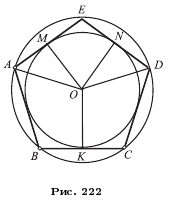
\includegraphics{mppics/ris-222}
\caption{}\label{1938/ris-222}
\end{wrapfigure}

1) Проведём окружность через какие-нибудь три соседние вершины $A, B$ и $C$ (рис.~\ref{1938/ris-222}) правильного многоугольника $ABCDE$ и докажем, что она пройдёт через следующую, четвёртую вершину $D$.
Опустим из центра $O$ перпендикуляр $OK$ на хорду $BC$ и соединим $O$ с $A$ и $D$.
Повернём четырёхугольник $ABKO$ вокруг стороны $OK$ так, чтобы он упал на четырёхугольник $ODCK$.
Тогда $KB$ пойдёт по $KC$ (вследствие равенства прямых углов при точке $K$), 
$B$ упадёт в $C$ (так как хорда $BC$ делится в точке $K$ пополам), 
сторона $BA$ пойдёт по $CD$ (вследствие равенства углов $B$ и $C$)
и, наконец, точка $A$ упадёт в $D$ (вследствие равенства сторон $BA$ и $CD$).
Из этого следует, что $OA$ совместится с $OD$, и, значит, точки $A$ и $D$ одинаково удалены от центра;
поэтому вершина $D$ должна лежать на окружности, проходящей через $A, B$ и $C$.
Точно так же докажем, что эта окружность, проходя через три соседние вершины $B, C$ и $D$, пройдёт через следующую вершину $E$, и~т.~д.;
значит, она пройдёт через все вершины многоугольника.

2) Из доказанного следует, что стороны правильного многоугольника всегда можно рассматривать как равные хорды одной окружности;
но такие хорды одинаково удалены от центра;
значит, все перпендикуляры $OM$, $ON$ и~т.~д., опущенные из $O$ на стороны многоугольника, равны между собой, и потому окружность, описанная радиусом $OM$ с центром в точке $O$, будет вписанной в многоугольник $ABCDE$.

\paragraph{}\label{1938/216}
\so{Следствие}.
Из предыдущего видно, что две окружности, описанная около правильного многоугольника и вписанная в него, имеют один и тот же центр.
Так как этот общий центр одинаково удалён от всех вершин многоугольника, то он должен лежать на срединном перпендикуляре, восстановленным к любой стороне многоугольника, а будучи одинаково удалён от сторон каждого угла, он должен находиться на его биссектрисе.
Поэтому, чтобы найти центр окружности, описанной около правильного многоугольника или вписанной в него, достаточно определить точку пересечения двух срединных перпендикуляров, восстановленных к сторонам многоугольника, или двух биссектрис углов, или одного срединного перпендикуляра с биссектрисой.

Легко заметить, что срединные перпендикуляры, восстановленные к сторонам правильного многоугольника, а также биссектрисы всех углов правильного многоугольника являются его осями симметрии.

\paragraph{}\label{1938/217}
\so{Определения}.
Общий центр окружностей, описанной около правильного многоугольника и вписанной в него, называется центром этого многоугольника, радиус вписанной окружности — \rindex{апофема}\textbf{апофемой} его.

Угол, составленный двумя радиусами, проведёнными к концам какой-нибудь стороны правильного многоугольника, называется центральным углом.
Центральных углов в многоугольнике столько, сколько сторон;
все они равны, как измеряющиеся равными дугами.

Так как сумма всех центральных углов равна $360\degree$, то в правильном $n$-угольнике каждый из них равен $\tfrac{360\degree}n$;
так, центральный угол правильного шестиугольника равен $\tfrac{360\degree}6\z=60\degree$, правильного восьмиугольника равен $\tfrac{360\degree}8 = 45\degree$ и так далее.

Так как сумма всех внутренних углов $n$-угольника (§~\ref{1938/82}) равна $180\degree\cdot(n-2)$, то каждый внутренний угол правильного $n$-угольника равен
\[\frac{180\degree\cdot(n-2)}{n}\]

Например, у правильного восьмиугольника внутренний угол равен
\[\frac{180\degree\cdot(8-2)}{8}=\frac{6}{8}\cdot 180\degree=\frac{3}{4}\cdot 180\degree=135\degree.\]

\paragraph{}\label{1938/218}
\so{Теорема}.
\textbf{\emph{Правильные $n$-угольники подобны, а стороны их относятся как радиусы или апофемы.}}

\begin{figure}[h!]
\centering
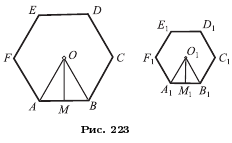
\includegraphics{mppics/ris-223}
\caption{}\label{1938/ris-223}
\end{figure}

1) Чтобы доказать подобие (рис.~\ref{1938/ris-223}) правильных $n$-угольников $ABCDEF$ и $A_1B_1C_1D_1E_1F_1$, достаточно обнаружить, что у них углы равны и стороны пропорциональны.

Углы $n$-угольников равны, так как каждый из них содержит одно и то же число градусов, а именно: $\frac{180\degree\cdot(n-2)}{n}$.
Так как 
\[AB=BC = CD=\dots,
\quad\text{и}\quad A_1B_1=B_1C_1 = C_1D_1=\dots,\]
то, очевидно, что
\[\frac{AB}{A_1B_1}=\frac{BC}{B_1C_1} = \frac{CD}{C_1D_1}=\dots;\]
то есть у таких $n$-угольников стороны пропорциональны.

2) Пусть $O$ и $O_1$ (рис.~\ref{1938/ris-223}) будут центры данных $n$-угольников, $OA$ и $O_1A_1$ — их радиусы, $OM$ и $O_1M_1$ — апофемы.
Треугольники $OAB$ и $O_1A_1B_1$ подобны, так как углы одного соответственно равны углам другого.

Из подобия их следует:
\[\frac{AB}{A_1B_1}=\frac{OA}{O_1A_1} = \frac{OM}{O_1M_1}\]

\smallskip
\so{Следствие}.
Так как периметры подобных многоугольников относятся как соответственные стороны (§~\ref{1938/172}), то \emph{периметры правильных $n$-угольников относятся как радиусы или как апофемы.}

%215(1996)+264(1914) симметрия правильных многугов

\paragraph{}\label{1938/219}
\so{Задача}.
\emph{Вычислить сторону вписанного в круг:
1) квадрата;
2) правильного шестиугольника;
3) правильного треугольника.}

\begin{wrapfigure}{r}{38mm}
\centering
\includegraphics{mppics/ris-224}
\caption{}\label{1938/ris-224}
\end{wrapfigure}

Условимся обозначать длину стороны правильного $n$-угольника буквой $a_n$, а его периметр — буквой $p_n$.

Формулы для сторон вписанного квадрата, шестиугольника и треугольника можно легко получить из рассмотрения рис.~\ref{1938/ris-224}—\ref{1938/ris-226}.

1) На рис.~\ref{1938/ris-224} проведены два взаимно перпендикулярных диаметра $AC$ и $BD$ и последовательные концы их соединены хордами;
от этого получился вписанный квадрат $ABCD$.


Из прямоугольного $\triangle AOB$ находим:
\[AB^2=AO^2+OB^2=2R^2.\]
откуда
\[a_4=R\sqrt2.\]

\paragraph{}\label{1938/220}
2) На рис.~\ref{1938/ris-225} построена хорда, соответствующая центральному углу в $60\degree$ (сторона правильного вписанного шестиугольника).

\begin{wrapfigure}{r}{38mm}
\vskip-4mm
\centering
\includegraphics{mppics/ris-225}
\caption{}\label{1938/ris-225}
\end{wrapfigure}

Так как у равнобедренного $\triangle AOB$ каждый из углов $A$ и $B$ равен \[\frac{180\degree-60\degree} 2 = 60\degree,\] то $\triangle AOB$ есть равноугольный и, следовательно, равносторонний;
значит:
\[AB=AO,\quad\text{то есть}\quad a_6 = R.\]
Отсюда мы получаем простой способ деления окружности на шесть равных частей.

\paragraph{}\label{1938/221}
3) На рис.~\ref{1938/ris-226} окружность разделена на шесть равных частей, и точки деления через одну последовательно соединены хордами, отчего образовался вписанный равносторонний треугольник $ABC$.

\begin{wrapfigure}{r}{38mm}
\centering
\includegraphics{mppics/ris-226}
\caption{}\label{1938/ris-226}
\end{wrapfigure}

Проведя хорду $AD$, получаем прямоугольный треугольник $ABD$ (угол $BAD$ как вписанный, опирающийся на диаметр, есть прямой).
Из $\triangle ABD$ находим:
\[AB=\sqrt{BD^2-AD^2},\]
то есть
\[a_3=\sqrt{(2R)^2-R^2}\]
и, значит,
\[a_3=R\cdot \sqrt3.\]

\paragraph{}\label{1938/222}
\so{Задача}.
\emph{Вписать в данный круг правильный десятиугольник и определить его сторону в зависимости от радиуса.}

\begin{wrapfigure}{r}{45mm}
\centering
\includegraphics{mppics/ris-227}
\caption{}\label{1938/ris-227}
\end{wrapfigure}

Предварительно докажем одно важное свойство правильного 10-угольника.
Пусть хорда $AB$ (рис.~\ref{1938/ris-227}) есть сторона правильного 10-угольника.
Тогда угол $AOB$ равен $36\degree$ , а каждый из углов $A$ и $B$ содержит по $\tfrac12(180\degree-36\degree)$, то есть
по $72\degree$.
Разделим угол $A$ пополам прямой $AC$.
Каждый из углов, образовавшихся при точке $A$, равен $36\degree$;
следовательно, $\triangle ACO$, имея два равных угла, есть равнобедренный, то есть $AC=CO$, $\triangle ABC$ также равнобедренный, потому что $\angle B = 72\degree$ и $\angle ACB = 180\degree- 72\degree- 36\degree = 72\degree$;
следовательно, $AB=AC=CO$.
По свойству биссектрисы угла треугольника (§~\ref{1938/186}) можно написать:
\[\frac{AO}{AB}=\frac{OC}{CB}.
\eqno(1)\]
Заменив $AO$ и $AB$ равными им отрезками $OB$ и $OC$, получим:
\[\frac{OB}{OC}=\frac{OC}{CB}, \eqno(2)\]
то есть радиус $OB$ разделён в точке $C$ в среднем и крайнем отношении (§~\ref{1938/209}), причём $OC$ есть его б\'{о}льшая часть.
Но $OC$ равна стороне правильного вписанного 10-угольника;
значит, \emph{сторона правильного вписанного 10-угольника равна б\'{о}льшей части радиуса, разделённого в среднем и крайнем отношении.}

\begin{wrapfigure}{R}{45mm}
\centering
\includegraphics{mppics/ris-228}
\caption{}\label{1938/ris-228}
\end{wrapfigure}

Теперь задача решается легко:

1) Делят радиус круга (например, $OA$, рис.~\ref{1938/ris-228}) в среднем и крайнем отношении%(§~\ref{1938/209})
;
затем, дав циркулю раствор, равный б\'{о}льшей части радиуса, откладывают им по окружности дуги, одна за другой, и точки деления последовательно соединяют хордами.

2) Обозначив буквой $x$ длину стороны правильного вписанного 10-угольника, мы можем пропорцию (2) переписать так:
\[\frac Rx=\frac x{(R-x)},\]
откуда
\[x^2-Rx-R^2=0.\]

Решив это квадратное уравнение, найдём:
\[x=a_{10}=R\cdot\tfrac{\sqrt5-1}{2}\approx R \cdot  0{,}61803\dots\]

\paragraph{}\label{1938/223}
\mbox{\so{Замечания}.}
1) Чтобы вписать в данный круг правильный пятиугольник, делят окружность на 10 равных частей (как указано выше) и точки деления соединяют через одну хордами.

2) Из равенства
\[\tfrac16-\tfrac1{10}=\tfrac5{30}-\tfrac3{30}=\tfrac2{30}=\tfrac1{15}\]
видно, что если из $\tfrac16$ части окружности вычесть $\tfrac1{10}$ её часть, то остаток будет равен $\tfrac1{15}$ окружности.
Это даёт нам простой способ вписать в окружность правильный 15-угольник, так как делить окружность на 6 и на 10 равных частей мы умеем.

\begin{wrapfigure}{r}{35mm}
\centering
\includegraphics{mppics/ris-229}
\caption{}\label{1938/ris-229}
\end{wrapfigure}

3) Чтобы построить пятиконечную звезду (рис.~\ref{1938/ris-229}), делят окружность на 10 равных частей и какую-нибудь из точек деления соединяют хордами с другими точками деления через три (как указано на рисунке).

\paragraph{}\label{1938/224}
\mbox{\so{Задача}.}
\emph{Удвоить число сторон правильного вписанного $n$-угольника.}

В этом сокращённом выражении подразумеваются две задачи:

1) по данному правильному вписанному $n$-угольнику \so{построить} правильный $2n$-угольник, вписанный в ту же окружность;

2) \so{вычислить сторону} этого $2n$-угольника по данной стороне данного $n$-угольника и данному радиусу круга.

\begin{wrapfigure}{R}{45mm}
\centering
\includegraphics{mppics/ris-230}
\caption{}\label{1938/ris-230}
\end{wrapfigure}

1) Пусть $AB$ (рис.~\ref{1938/ris-230}) есть сторона правильного вписанного $n$-угольника и $O$ — центр круга.
Проведём $OC\perp AB$ и соединим $A$ с $C$.
Дуга $AB$ делится в точке $C$ пополам, следовательно, хорда $AC$ есть сторона правильного вписанного $2n$-угольника.

2) В $\triangle ACO$ угол $O$ всегда острый (так как дуга $ACB$ всегда меньше полуокружности, и, следовательно, половина её, дуга $AC$, меньше четверти окружности);
поэтому (§~\ref{1938/194})
\[AC^2=OA^2+OC^2-2OC\cdot OD,\]
то есть
\[a_{2n}^2=R^2+R^2-2R\cdot OD=2R^2-2R\cdot OD.\]

Из прямоугольного $\triangle AOD$ определим катет $OD$:
\begin{align*}
OD&=\sqrt{AO^2-AD^2}=
\\
&=\sqrt{R^2-(\tfrac{a_n}2)^2}=
\\
&=\sqrt{R^2-\tfrac{a_n^2}4}.
\end{align*}
Следовательно,
\[a_{2n}^2=2R^2-2R\sqrt{R^2-\frac{a_n^2}4}.\]
Такова формула удвоения числа сторон правильного вписанного многоугольника (из неё сторону $a_{2n}$ получим посредством извлечения квадратного корня).

\smallskip
\so{Пример}.
Вычислим сторону правильного 12-угольника.
Для простоты примем, что $R=1$ (и, следовательно, $a_6 = 1$).
\begin{align*}
a_{12}^2&=2-2\sqrt{1-\tfrac14}=
\\
&=2-2\sqrt{\tfrac34}=
\\
&=2-\sqrt{3},
\end{align*}
откуда
\[a_{12}=\sqrt{2-\sqrt3}\approx 0{,}517\dots\]
Так как стороны правильных $n$-угольников пропорциональны их радиусам (§~\ref{1938/218}), то при радиусе, равном не единице, а какому-нибудь числу $R$, для стороны правильного 12-угольника получим такую формулу:
\[a_{12}=R\cdot \sqrt{2-\sqrt3}\approx R\cdot 0{,}517\dots\]

\paragraph{На сколько равных частей можно делить окружность с помощью циркуля и линейки?}\label{1938/225}
Применяя указанные в предыдущих задачах способы, мы можем с помощью циркуля и линейки делить окружность на такое число равных частей (и, следовательно, вписывать в окружность правильные многоугольники с таким числом сторон), которое заключается в следующей таблице:
\begin{align*}
3,&&3\cdot 2,&&3\cdot2\cdot2,&&\text{вообще}&&3\cdot 2^n,&
\\
4,&&4\cdot 2,&&4\cdot2\cdot2,&&\text{—\textquotedbl—\ \ }&&2^n,&
\\
5,&&5\cdot 2,&&5\cdot2\cdot2,&&\text{—\textquotedbl—\ \ }&&5\cdot 2^n,&
\\
15,&&15\cdot 2,&&15\cdot2\cdot2,&&\text{—\textquotedbl—\ \ }&&15\cdot 2^n.&
\end{align*}

Немецкий математик Гаусс (живший в 1777—1855 годах) доказал, что посредством циркуля и линейки можно делить окружность на такое число равных частей, которое, будучи простым, выражается формулой $2^{2^n} + 1$.
Например, можно разделить окружность на 17 равных частей и на 257 равных частей, так как 17 и 257 простые числа вида $2^{2^n} + 1$ 
($17 = 2^{2^2} + 1$;
$257 = 2^{2^3} + 1$).
Доказательство Гаусса выходит за пределы элементарной математики.

Доказано также, что с помощью линейки и циркуля окружность можно делить на такое составное число равных частей, в состав которого не входят никакие иные простые множители, кроме:
1) множителей вида $2^{2^n} + 1$ при условии, что все эти множители различны 
и 
2) множителя 2 в какой угодно степени.

Например, в окружность с помощью циркуля и линейки можно вписать правильный 170-угольник ($170 = 2 \cdot 5 \cdot 17 = 2 \cdot (2^2 + 1) \cdot (2^{2^2} +1)$),
но нельзя вписать правильный 9-угольник (хотя множитель 3 имеет вид $2^{2^n} + 1$, но в составе 9 он повторяется).

На всякое иное число равных частей окружность может быть разделена \so{приближённо}.
Пусть, например, требуется разделить окружность на 7 равных частей (или вписать правильный семиугольник).
Тогда предварительно вычислим величину центрального угла,
$\frac{360\degree}7=51\tfrac37\degree$.
Построить точно такой угол мы не можем, но по транспортиру приблизительно можем отложить при центре угол в $51\degree$ и тогда получим приблизительно $\tfrac17$ часть окружности.

\subsection*{Упражнения}

\begin{enumerate}

\item
Составить формулу для стороны правильного вписанного 24-угольника.

\item
Составить формулу для сторон правильных вписанных восьмиугольника и 16-угольника.

\item
Составить формулу для сторон правильных описанных треугольника и шестиугольника.

\item
Пусть $AB, BC$ и $CD$ будут три последовательные стороны правильного многоугольника, имеющего центр в $O$.
Доказать, что если продолжим стороны $AB$ и $CD$ до взаимного пересечения в точке $E$, то четырёхугольник $OAEC$ может быть вписан в окружность.

\item
Доказать, что:
1) всякий вписанный равносторонний многоугольник — правильный;
2) всякий описанный равноугольный многоугольник — правильный.

\item
Доказать, что:
1) каждый правильный $n$-угольник имеет $n$ осей симметрии, причём все эти оси симметрии проходят через его центр;
2) для многоугольника с чётным числом сторон центр многоугольника является центром его симметрии.

\item
Доказать, что две диагонали правильного пятиугольника, не исходящие из одной вершины, пересекаясь, делятся в среднем и крайнем отношении.

\smallskip
\so{Указание}.
Пусть $ABCDE$ — правильный пятиугольник, $AC$ и $BE$ — его диагонали, $F$ — точка их пересечения.
$\triangle ABC \sim \triangle ABF$ и~т.~д.

\item
На данной стороне построить:
1) правильный восьмиугольник;
2) правильный 10-угольник.

\item
Срезать от данного квадрата углы так, чтобы образовался правильный восьмиугольник.

\item
В данный квадрат вписать равносторонний треугольник, помещая одну из его вершин или в вершине квадрата, или в середине какой-либо стороны.

\item
Вписать в равносторонний треугольник другой равносторонний треугольник, стороны которого были бы перпендикулярны к сторонам данного.

\item
Построить углы в $18\degree$, $30\degree$, $72\degree$, $75\degree$.

\item
Около окружности описан какой-нибудь правильный многоугольник.
Пользуясь им, вписать в эту окружность правильный многоугольник, имеющий вдвое более сторон, чем описанный.

\end{enumerate}